\chapter{Covid}\label{chapter:Covid}
\addcontentsline{toc}{chapter}{Covid}
In questo capitolo verrà introdotto il virus covid, la funzione della proteina spike e vedremo una conformazione della stessa. 


\section{Covid-19}\label{sec:cap_sec_subsec}
%http://mjpath.org.my/2020/v42n1/properties-of-coronavirus.pdf
Le informazioni in questa sezione sono state prese da \cite{ProprietàCovid}.
I coronavirus sono stati scoperti negli anni 60 e da allora i coronavirus sugli umani sono stati identificati a partire dal SARS-CoV nel 2002. La pandemia da Covid-19 
è causata da un nuovo ceppo virale chiamato SARS-CoV-2, un virus a singola elica di RNA della famiglia \emph{coronaviridae}. Le specie patogene individuate nel tempo
sono SARS-CoV, MERS-CoV e appunto SARS-CoV-2 di ordine nidovirale della famiglia coronaviridae e sotto famiglia ortocoronavirinae, e tutte hanno un aspetto a forma
di corona solare. Dei 4 generi di coronavirus ($\alpha, \beta, \gamma, \delta$) fa parte dei $\beta-CoV$ e mostra molte somiglianze con 2 coronavirus derivati dai 
pipistrelli. 

SARS-CoV e MERS-CoV hanno avuto origine nei pipistrelli, e sembra che sia così anche per SARS-CoV-2. Era gia stata dimostrata in precedenza la possibilità che un host
intermedio facilitasse l'emergere del virus negli umani; dopodiché il contagio tra uomo e uomo può avvenire attraverso contatti ravvicinati con goccioline respiratorie, 
oppure con con diretto con infetti e o per contatto con oggetti e superfici contaminate.

Il genoma del virus contiene 4 strutture proteiche: la proteina spike; la membrana; l'envelope; la nucleocapside. La proteina spike media l'attaccamento del virus ai 
recettori dell'ospite, ma la approfondiremo nella prossima sezione. La membrana è la proteina più abbondante e definisce la forma dell'involucro virale. La proteina 
envelope è la più piccola proteina appartenente alla struttura virilica, partecipa all'assemblaggio virale e al gemogliamento. La proteina nucleocapside è l'unica che 
si lega al genoma del RNA ed è coinvolta nel assemblaggio virale e nel germogliamento. 

La replicazione del virus inizia con l'attaccamento e l'ingresso; l'attaccamento del virus alla cellula ospite avviene tra la proteina spike e il recettore specifico. 
Una volta che si viene a creare il legame, il virus entra nel citosol della cellula ospite. Dopodiché avviene la traduzione del gene per la replicazione dal RNA 
genomico e quindi poi la traduzione e l'assemblaggio dei processi di replicazione virale. Una volta conclusa questa fase avviene l'incapsulamento che porta alla 
formazione del virus maturo. Una volta completato il processo di assemblaggio viene trasportato sulla superficie cellulare e rilasciato per esocitosi.

Prima dell'epidemia del SARS-CoV erano già stati indivuduati due tipologie di coronavirus nell'uomo che però erano visti come le cause del raffreddore. Con la comparsa
nel 2012 di MERS-CoV e l'attuale SARS-CoV-2 è necessario studiare e comprendere appieno quelle che sono le proprietà e le caratteristiche di questo virus. 

\subsection{Storia}\label{subsec:es_subsec}
%https://www.simg.it/Riviste/rivista_simg/2020/02_2020/3.pdf
%https://www.epicentro.iss.it/coronavirus/sars-cov-2
Le informazioni in questa sezione sono state prese da \cite{StoriaCovid} e da \\
\cite{ReportCovid}.
Ha avuto inizio il 31 Dicembre del 2019 quando l'OMS (Organizzazione Mondiale della Sanità) è stata informata di casi di polmonite di eziologia sconosciuta nella città di Wuhan provincia di Hubei Cina. Il nuovo corona virus è stato ufficialmente annunciato il 7 gennaio del 2020 e tre giorni dopo è stata resa pubblica la sequenza genomica. Sono state poi rilasciate altre sequenze genomiche, le quali tutte suggerivano la presenza di un virus strettamente legato al SARS-CoV. 

L'11 Febbraio del 2020 l'OMS ha definito la nuova polmonite indotta da coronavirus come malattia da corona virus 2019. Allo stesso tempo la Commissione internazionale di classificazione dei virus ha annunciato che il virus nominato provvisoriamente come 2019-nCoV veniva nominato come grave sindrome respiratoria acuta SARS-CoV2. Dopo che il patogeno è stato valutato sulla base della filogenesi, della tassonomia e della pratica consolidata, è stato definito un forte legame con il precedente SARS-CoV. 

L'inizio della pandemia è avvenuto quindi a Wuhan in Cina. In Italia si sviluppo poi un focolaio autoctono che poi si è diffuso progressivamente in tutto il paese e in particolare nelle regioni del nord. Successivamente il virus si espanse in Europa e nel resto del mondo. L'OMS dichiarò l'inizio della pandemia l'11 Marzo del 2020, è poi storia di ogni giorno della pandemia che ha raggiunto milioni di persone. Si ritiene che comunque il tasso di mortalità del virus sia di circa il 3.5\%.  

\subsection{Caratteristiche genetiche}\label{subsec:es_subsec}
I coronavirus sono sferici con un diametro di circa 125nm con punte a forma di clava che sporgono dalla superficie del virus che danno l'aspetto di una corona solare. 

\begin{figure}
	\centering
	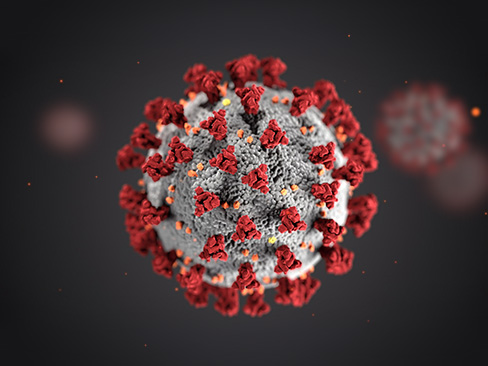
\includegraphics[width=0.4\textwidth]{Immagini/coronavirus.png}
	\caption{Molecola di un coronavirus}
	\label{fig:Amminoacido}
\end{figure}

All'interno dell'involucro troviamo una simmetria elicoidale dei nucleocapsidi, che in realtà è molto rara tra i virus a RNA a senso positivo. I CoV sono classificati nell'ordine Nidovirales, famiglia Coronaviriade e sotto famiglia Orthocoronavirinae. Nidovirales è un ordine di virus a RNA a singolo filamento positivo. Essi si distinguono da altri virus a RNA per la loro lunghezza e complessità del genoma e per la presenza di una struttura a corona di proteine sulla superficie virale. Il loro genoma contiene diversi geni che codificano proteine non strutturali coinvolte nella replicazione e nella trascrizione del virus nonché geni che codificano le proteine strutturali che costituiscono il virus stesso. Gli Nidovirales includono quattro famiglie virali:
\vspace{10pt}
\begin{itemize}
	\item Coronaviridae,
	\vspace{5pt}
	\item Arteriviridae,
	\vspace{5pt}
	\item Roniviridae,
	\vspace{5pt}
	\item Mesoniviridae.
\end{itemize}

La famiglia Coronaviridae è una famiglia di virus a RNA a singolo filamento positivo che causano malattie respiratorie e gastroenteriti in animali e in alcuni casi anche nell'uomo. I coronavirus sono stati scoperti per la prima volta negli anni '60, e devono il loro nome alla loro forma a corona, che deriva dalle protuberanze sulla loro superficie virale. La famiglia Coronaviridae è suddivisa in quattro generi:
\vspace{10pt}
\begin{itemize}
	\item Alphacoronavirus,
	\vspace{5pt}
	\item Betacoronavirus,
	\vspace{5pt}
	\item Gammacoronavirus,
	\vspace{5pt}
	\item Deltacoronavirus.
\end{itemize}

Un'analisi filogenetica ha inserito SARS-CoV2 sotto il sottogenere Sarbecovirus del genere Betacoronavirus. 

Le 4 proteine strutturali, citate in precedenza, sono richieste dalla maggior parte dei CoV per produrre una particella virale strutturalmente completa suggerendo che alcuni Cov possono codificare proteine aggiuntive con funzioni in sovrapposizione compensative.

\subsection{RNA polimerasi}\label{subsec:es_subsec}
%https://www.unisr.it/news/2020/7/rna-polimerasi-la-fotocopiatrice-distratta-di-sars-cov-2
Le informazioni in questa sezione sono prese da \cite{RNApolimerasi}
La fase di ingresso del virus viene approfondita nella prossima sezione, ora pensiamo a cosa succede quando è all'interno. Una volta all'interno della parte acquosa della cellula ospite, chiamata citosol, il virus si "scompone" rilasciando il suo contenuto; un insieme di proteine e materiale genetico. L'uomo conserva l'informazione genetica, ovvero quella che ci permette di costruire le cellule, nelle molecole di DNA, il virus utilizza una singola molecola di RNA. L'RNA è presente anche nell'uomo, ma che principalmente viene utilizzato per la costruzione delle proteine. 

Una volta che il coronavirus ha infettato una cellula, il suo scopo è quello di far si che si costruiscano nuove copie dello stesso in modo da avere una discendenza in grado di espandere la specie. Tutto quello che è presente nella singola cellula infetta deve essere "copiato" e assemblato per formare nuovi vironi. Per ottenere la "copia" è necessario replicare il materiale genetico "RNA" del virus stesso. Il meccanismo che permette di far ciò si chiama RNA polimerasi, ovvero un enzima che è in grado di formare lunghe catene di RNA. In modo specifico l'RNA polimerasi di SARS-CoV-2 si chiama RdRP (RNA polimerasi RNA-dipendente). 

\begin{figure}
	\centering
	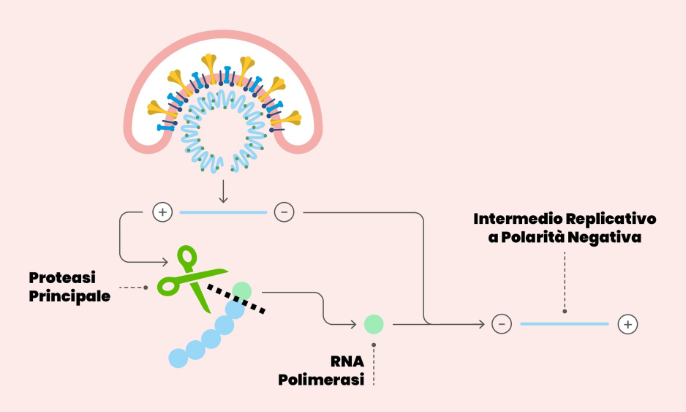
\includegraphics[width=0.6\textwidth]{Immagini/RNA_polimerasi.png}
	\caption{Principio del RNA polimerasi}
	\label{fig:Amminoacido}
\end{figure}

Esso viene però definito "distratto", infatti ogni volta che effettua la "copia" del materiale genetico originale commette degli errori, di conseguenza la copia presenta delle differenze. Le seguenti differenze non sono altro che mutazioni che si ripercuotono sulla struttura delle proteine del virus e sulla loro funzione. Non a caso si sono sentite varie varianti presenti come Delta, Omicron, etc... Quello che succede è che l'RNA polimerasi ha fatto una copia del genoma virale e ha cambiato una base di RNA. In ogni caso le mutazioni hanno conseguenze sul virus, possono essere neutre, vantaggiose o svantaggiose. Una mutazione può iniziare a circolare se essa da un vantaggio per il suo ciclo vitale, questo può significare essere più abile nell'infettare, ma provocare meno danni nell'organismo ospite, dato che un virus altamente letale è destinato a scomparire per mancanza di ospiti.

\section{Glicoproteina Spike}\label{sec:cap_sec_subsec}
%https://www.frontiersin.org/articles/10.3389/fimmu.2020.576622/full#f2
Le informazioni in questo sezione sono state prese da \cite{GlicoproteinaSpike}
La glicoproteina spike svolge un ruolo essenziale nell'attaccamento, nella fusione e nell'ingresso del virus nella cellula ospite. Una caratteristica dei coronavirus è quella di accedere alle cellule ospiti e poi dare inizio all'infezione attraverso la fusione delle membrane virali alle cellule. La fusione della membrana viene mediata dalla membrana di tipo 1 della glicoproteina spike e dal recettore affine della cellula ospite. Essendo in una posizione superficiale nella struttura del virus, ciò la rende un bersaglio diretto per le risposte immunitarie dell'ospite rendendola anche il principale bersaglio degli anticorpi. Data la sua importanza nella replicazione e fusione virale è al centro della maggior parte delle strategie vaccinali e degli interventi terapeutici. 

La glicoproteina Spike viene sintetizzata come precursore di una poliproteina sul reticolo endoplasmatico ruvido (RER). Il precursore non processato ospita una sequenza segnale del reticolo endoplasmatico (ER) situato nel terminale N, che indirizza la glicoproteina alla membrana RER. Durante la sintesi vengono aggiunte catene laterali di oligosaccaridi ad alto contenuto di mannosio. Poco dopo la sintesi i monomeri della glicoproteina trimerizzano, il che può facilitare il trasporto dall'ER al complesso di Golgi. Il complesso di Golgi è un organulo di composizione lipo-proteica con una delicata struttura nella cellula in posizione paranucleare che si occupa di rielabolare, selezionare ed esportare i prodotti del reticolo endoplasmatico. All'interno del complesso di Golgi la glicoproteina spike viene scissa proteoliticamente dalla furina cellulare o da proteasi simili in S1 e S2. La subunità di superficie S1, che attacca il virus al recettore della superficie della cellula ospite e la subunità S2 che media la fusione delle membrane cellulari alla cellula ospite. Anche dopo la fase di scissione le subunità S1 e S2 rimangono associate attraverso interazioni non covalenti in uno stato di profusione metastabile. La scissione è però necessaria per l'infettività virale ed è anche necessaria per un efficacie infezione delle cellule polmonari. Un segnale di recupero dell'ER costituito da un motivo conservato KxHxx assicura che la proteina matura si accumuli vicino al compartimento intermedio di Golgi dove guidata dall'interazione con la proteina di membrana (M) partecipano all'assemblaggio delle particelle virali. Una frazione delle proteine mature viaggia attraverso via secretoria fino alla membrana plasmatica, dove può mediare la fusione di cellule infette con cellule non infette per formare cellule giganti multinucleate.

\subsection{Struttura della proteina e funzione}\label{subsec:es_subsec}
Come accenato nei precedenti paragrafi la glicoproteina spike svolge un ruolo fondamentale nell'infezione virale e nella patogenesi. Essa è un trimero fortemente glicosilato. La subunità S1 è composta da 672 amminoacidi ed organizzata in 4 domini: un dominio N-terminale; un dominio C-terminale, noto anche come dominio di legame; due sottodomini SD1 e SD2. Mentre la subunità S2 è composta da 588 amminoacidi e contiene un peptide di fusione idrofobica N-terminale, due ripetizioni eptade, un dominio transmembrana e una coda citoplasmatica.

Come una tipica proteina di fusione di classe I la glicoproteina spike condivide caratteristiche strutturali topologiche e meccaniche comuni con altre proteina di fusione di classe I come la glicoproteina dell'involucro dell'HIV e l'emoagglutinina del virus dell'influenza. Essa è una macchina coformazionale che media l'ingresso virale riorganizzando da uno stato non unliganded metastabile, attraverso uno stato intermedio ad uno stato post fusione stabile. Da quando è stata resa pubblica la struttura sono state scoperte numerose strutture per i frammenti di trimero della glicoproteina spike negli stati pre e post fusione. 

\begin{figure}
	\centering
	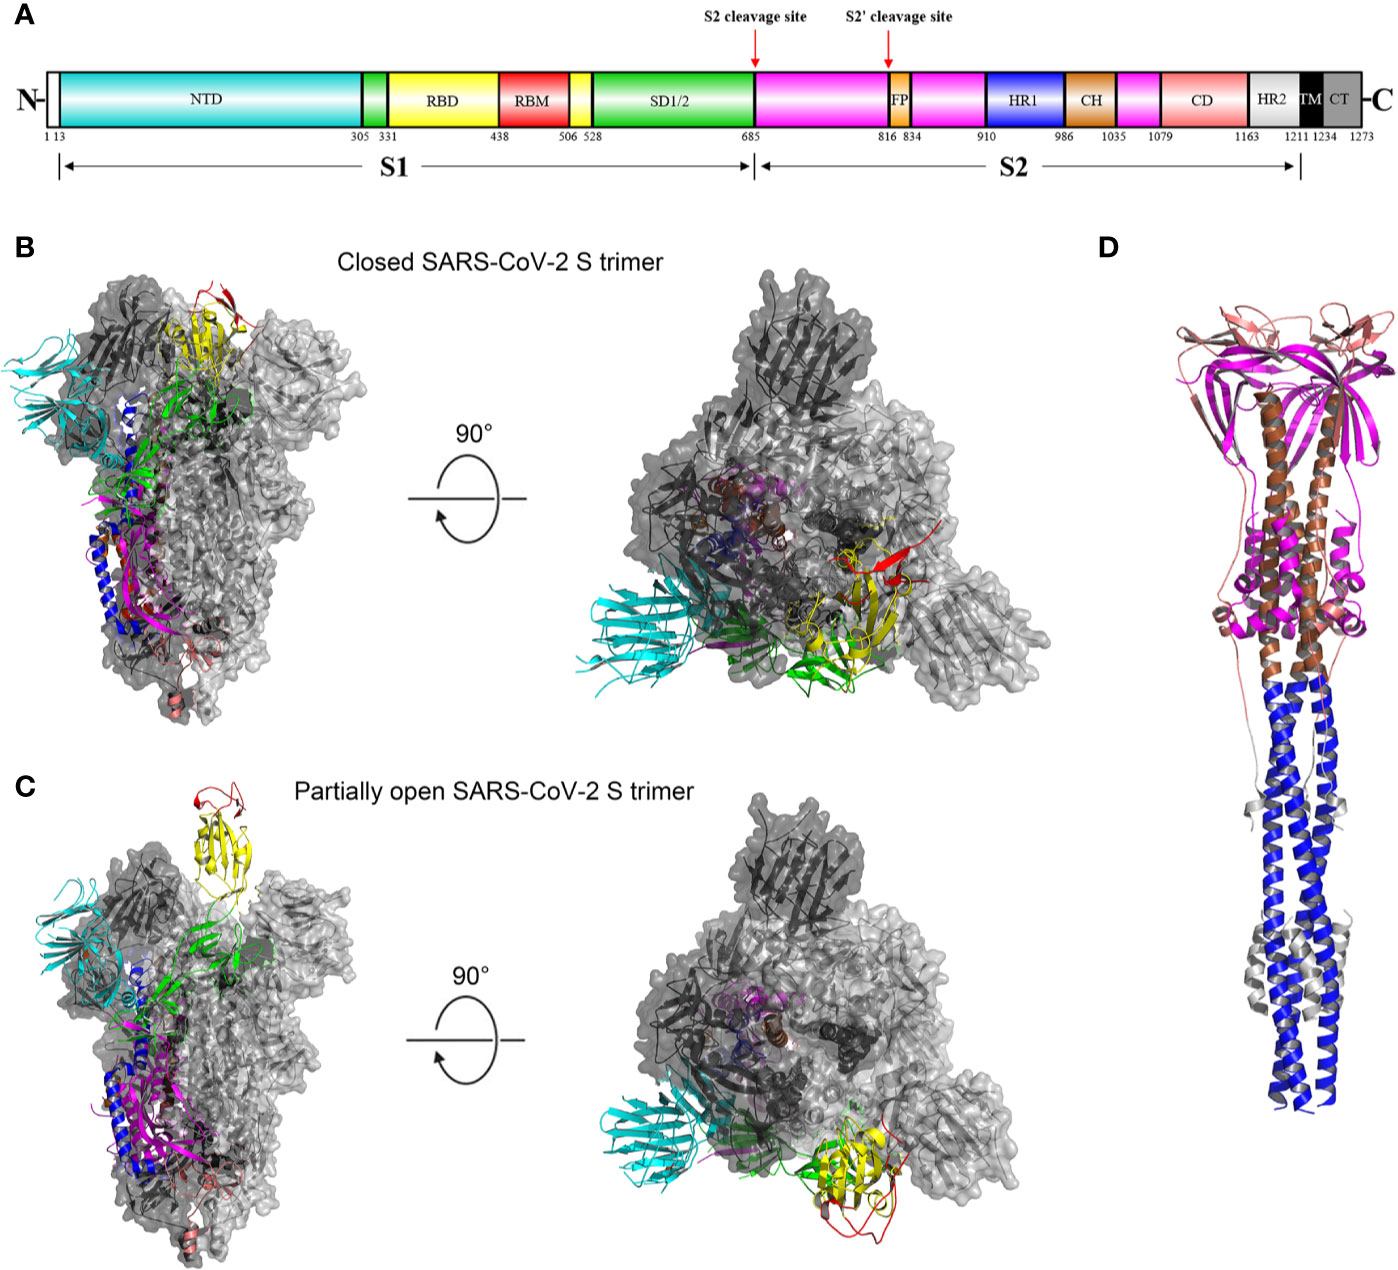
\includegraphics[width=0.7\textwidth]{Immagini/Composizione_strutturale.png}
	\caption{Struttura di massima della glicoproteina spike}
	\label{fig:StrutturaMassima}
\end{figure}

L'architettura di massima dell'ectodominio pre fusione della spike è stabilizzato da due mutazioni consecutive della prolina in due conformazioni determinate dalla microscopia crioelettronica a singola particella è un trimero con una sezione trasversale triangolare. La differenza strutturale tra queste due conformazioni risiede solo nella posizione di uno dei tre RDB. Quando tutti e tre gli RBD sono nella posizione giù il trimero risultante di ectodominio S assume una configurazione chiusa, in cui la superficie di legame del recettore dell'RBD S1 è sepolta tra i protomeri e non può essere accessibile dal suo recettore (Fig. \ref{fig:StrutturaCovid}B). Il trimero di ectodominio S con un singolo RBD nella posizione "up" assume una conformazione parzialmente aperta e rappresenta lo stato funzionale poiché la superficie di legame del recettore del RBD "up" può essere completamente esposta (Fig. \ref{fig:StrutturaCovid}C). La subunità S1 riposa mentre il trimero S2 stabilizzano quest'ultimo nella conformazione di pre fusione. Quando il trimero di ectodomionio adotta una conformazione parzialmente aperta l'RBD nella posizione "su" abolirà i contatti con la subunità S2 di un protomero adiacente, destabilizzando la conformazione parzialmente aperta. Ciò sarà vantaggioso per la dissociazione e faciliterà i riagganciamenti subiti per mediare l'ingresso virale. 

Le strutture di pre fusione del coronavirus umano senza due mutazioni consecutive della prolina rivelano solo una conformazione completamente chiusa. In particolare è noto che la pre fusione trimerica risiede principalmente in una configurazione chiusa che è conformazionalmente mascherata per eludere le neutralizzazioni mediate dagli anticorpi. Si può quindi pensare che le glicoproteine spike del covid-19 native su virioni maturi e infettivi che condividano una simile caratteristica di mascheramento conformazionale, nascondendo la superficie di legame del recettore.

\subsection{Scudo di glicani della glicoproteina spike}\label{subsec:es_subsec}
Come nominato in precedenza la proteina spike del SARS-CoV-2 è fortemente circondata da glicani N-legati che sporgono dalla superficie del trimero. Sono stati incontrati fino a 22 glicani N-legati che probabilmente svolgono un ruolo importante nel ripiegamento delle proteine e nell'invasione immunitaria dell'ospite come scudo glicano. Dei 22 potenziali disponibili per la glicosilazione, 14 vengono identificati come prevalentemente occupati da glicani di tipo complesso. I restanti invece risultano dominati da glicani di tipo oligomannosio che sono diversi da quelli fondati sulle glicoproteine dell'ospite. Per glicosilazione si intende una modifica della struttura della proteina da parte del complesso di Goigi, durante o in seguito ad un processo di sintesi proteica. Essa avviene per più motivi, uno dei quali è il raggiungimento del ripiegamento corretto, la può proteggere dall'attaccco di proteasi e aumenta la solubilità della molecola che viene dunque stabilizzata in tutti gli aspetti. Si può anche affermare che l'affinità di legame tra la proteina spike del SARS-CoV-2 e ACE2 non dipendono dalla glicosalinzione della stessa.

Quando i glicani specifici sono mappati sulla struttura di pre fusione dell'ectodominio della spike del SARS-CoV-2 il modello ha mostrato livelli sostanzialmente più elevati di superficie priva di glicani. Questo ci porta alla considerazione che la proteina spike del SARS-CoV-2 è ricoperta da uno scudo meno denso e quindi risulta essere una buona notizia per i potenziali vaccini. 

Nel caso di SARS-CoV-2, più recentemente è stato dimostrato che un potente anticorpo neutralizzante sia contro SARS-CoV che SARS-CoV-2, S309, riconosce un epitopo RBD contenente glicano altamente conservato. Queste osservazioni suggeriscono che le frazioni di carboidrati potrebberò essere immunogeniche ed evidenziano la necessità per gli immunogeni di mostrare i glicani importanti per il riconoscimento degli anticorpi neutralizzanti. Di conseguenza anche in questo caso è diventa fondamentale la ricerca in questo campo per i vaccini.

\section{RBD}\label{sec:cap_sec_subsec}
%https://www.ncbi.nlm.nih.gov/pmc/articles/PMC9581196/
Le informazioni in questa sezione sono state prese da \cite{RBDSpike}.
Diverse linee di ricerca hanno stabilito che l'enzima di conversione dell'angiotesina 2 (ACE2) è un recettore di ingresso per SARS-CoV-2. Interazioni dettagliate tra il SARS-CoV-2 RBD e il suo recettore sono state rivelate da diverse strutture in ACE2. Come detto nella sezione precedente le subunità S1 e S2 sono responsabili del legame del recettore e della fusione della membrana. La subunità S1 è costituita da un dominio N-terminale e un dominio di legame o RBD. Nello stato di pre fusione, la proteina S esiste come omotrimero e subisce grandi cambiamenti conformazionali per controllare l'esposizione e l'accessibilità del RBD.Tutto questo avviene mediante un meccanismo di "su" e "giù", la differenza sta nel rendere accessibile o inaccessibile il recettore. La struttura del nucleo RBD quando è lagata ad ACE2 è costituita da un foglio $\beta$ antiparallelo a cinque filamenti intrecciati con eliche e anelli di collegamento corti. 
\begin{figure}
	\centering
	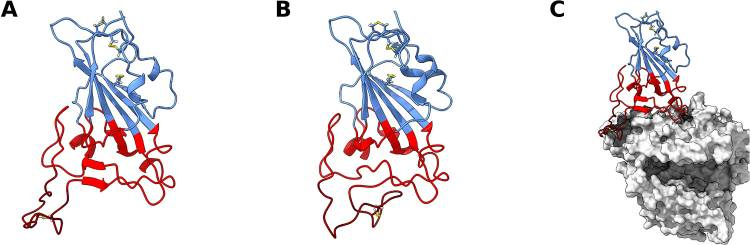
\includegraphics[width=0.7\textwidth]{Immagini/RBD_structure.png}
	\caption{Struttura del dominio di legame del recettore SARS-CoV-2, nella conformazione aperta (A) e chiusa (B). (C) rappresenta la struttura legata ad ACE2}
	\label{fig:RBDstructure}
\end{figure}

Questa struttura centrale del foglio $\beta$ è ulteriormente stabilizzata da 3 legami di di solfuro. Tra i filamenti centrali c'è una regione estesa contenente 2 filamenti $\beta$ corti, le eliche e gli anelli. Questa regione è il motivo legante il recettore (RBM) che contiene la maggior parte dei residui responsabili dell'interazione con ACE2. Quando complessato con ACE2, l'RBM si ripiega in una superficie concava che ospita l'$\alpha$-elica N-terinale di ACE2. E' proprio in questa superficie che diversi residui di RBM stabiliscono interazioni specifiche e non specifiche con i residui di ACE2. Dai dati disponibili riguardo alla struttura sembrerebbe che la struttura centrale sia abbastanza stabile, mentre l'RBM risulta molto dinamico e non definito strutturalmente, a meno che non sia legato ad altre proteine come ACE2. 

Durante il corso della pandemia sono state segnalate un numero significativo di mutazioni naturali della proteina Spike. Molte delle mutazioni sono state identificate nel RBD, alcune delle quali hanno dato origine a varianti virali. Si ritiene che molte di queste mutazioni RBD aumentino l'affinità di legame per ACE2 o riescono ad ingannare in modo migliore gli anticorpi monoclonali.  

I vaccini che sono stati elaborati nel corso della pandemia vanno proprio ad agire in questa zona tra RBD e ACE2, cercando di impedire che avvenga il contatto e che quindi impedire di conseguenza l'ingresso del virus all'interno dell'ospite.
